\documentclass[11pt]{article}

\usepackage{amssymb}
\usepackage{amsmath}
\usepackage{xcolor}
\usepackage{graphicx}

\usepackage{placeins}
\usepackage{hyperref}

\usepackage{listings}

% set the default code style
\lstset{
    frame=tb, % draw a frame at the top and bottom of the code block
    tabsize=4, % tab space width
    showstringspaces=false, % don't mark spaces in strings
    numbers=left, % display line numbers on the left
    commentstyle=\color{green}, % comment color
    keywordstyle=\color{blue}, % keyword color
    stringstyle=\color{red} % string color
}

\graphicspath{ {images/} }

\setlength\parindent{0pt}

\begin{document}

\title{Model Predictive Control}
\author{Philippe Weingertner}
\date{\today}
\maketitle

\tableofcontents

\section{Motion Control}

Motion Control deals with the last stage of an autonomous driving pipeline: the control module.
The input to the control module will be provided by the output of the path planning module via a set of waypoints to follow as close as possible.
The control module will have to provide the actuators commands (in our case steering angle and throttling; acceleration or deceleration) so that the automated driving comply with a set of rules:


\begin{itemize}
\item follow the planned waypoints as close as possible
\item drives smoothly
\item try to adjust the speed: as fast as a configurable reference when possible and driving more slowly during curves
\end{itemize}



\begin{figure}[h]
    \centering
    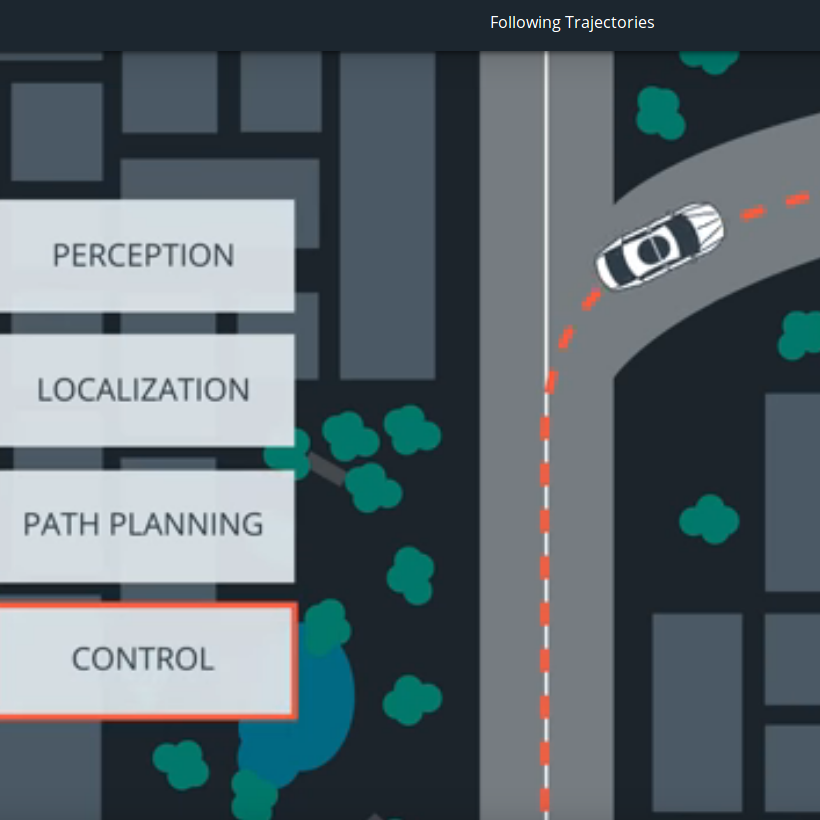
\includegraphics[width=0.5\textwidth]{pipeline}
    \caption{Autonomous Driving pipeline}
    \label{fig:pipeline}
\end{figure}

\section{Non linear optimization under constraints}

\subsection{Definition}

In its most generic form we are dealing with the following problem:

\begin{equation*}
\begin{aligned}
& \underset{x}{\text{minimize}}
& & f_0(x) \\
& \text{subject to}
& & lower_i \leq f_i(x) \leq upper_i, \; i = 1, \ldots, m.
\end{aligned}
\end{equation*}

Note that by setting $lower_i = upper_i $ we can define constraints as equalities as well.

\subsection{Example}

\begin{equation*}
\begin{array}{lc}
{\rm minimize \; }      &  x_1 * x_4 * (x_1 + x_2 + x_3) + x_3 \\
{\rm subject \; to \; } &  x_1 * x_2 * x_3 * x_4  \geq 25 \\
                        &  x_1^2 + x_2^2 + x_3^2 + x_4^2 = 40 \\
                        &  1 \leq x_1, x_2, x_3, x_4 \leq 5
\end{array}
\end{equation*}

\subsection{Solving with ipopt}

ipopt and cppad are used to solve non-linear minimization problems.
ipopt requires the computation of first order (Jacobians) and 2nd order derivatives (Hessians).
These derivatives will be computed automatically thanks to cppad: providing automatic differentiation services. \\
The previous example is solved with ipopt and CppAD here:
\url{https://www.coin-or.org/CppAD/Doc/ipopt_solve_get_started.cpp.htm}

\begin{lstlisting}[language=C++, caption={Simple example with ipopt}]


# include <cppad/ipopt/solve.hpp>

namespace {
     using CppAD::AD;

     class FG_eval {
     public:
          typedef CPPAD_TESTVECTOR( AD<double> ) ADvector;
          void operator()(ADvector& fg, const ADvector& x)
          {     assert( fg.size() == 3 );
               assert( x.size()  == 4 );

               // Fortran style indexing
               AD<double> x1 = x[0];
               AD<double> x2 = x[1];
               AD<double> x3 = x[2];
               AD<double> x4 = x[3];
               // f(x)
               fg[0] = x1 * x4 * (x1 + x2 + x3) + x3;
               // g_1 (x)
               fg[1] = x1 * x2 * x3 * x4;
               // g_2 (x)
               fg[2] = x1 * x1 + x2 * x2 + x3 * x3 + x4 * x4;
               //
               return;
          }
     };
}

bool get_started(void)
{     bool ok = true;
     size_t i;
     typedef CPPAD_TESTVECTOR( double ) Dvector;

     // number of independent variables (domain dimension for f and g)
     size_t nx = 4;
     // number of constraints (range dimension for g)
     size_t ng = 2;
     // initial value of the independent variables
     Dvector xi(nx);
     xi[0] = 1.0;
     xi[1] = 5.0;
     xi[2] = 5.0;
     xi[3] = 1.0;
     // lower and upper limits for x
     Dvector xl(nx), xu(nx);
     for(i = 0; i < nx; i++)
     {     xl[i] = 1.0;
          xu[i] = 5.0;
     }
     // lower and upper limits for g
     Dvector gl(ng), gu(ng);
     gl[0] = 25.0;     gu[0] = 1.0e19;
     gl[1] = 40.0;     gu[1] = 40.0;

     // object that computes objective and constraints
     FG_eval fg_eval;

     // options
     std::string options;
     // turn off any printing
     options += "Integer print_level  0\n";
     options += "String  sb           yes\n";
     // maximum number of iterations
     options += "Integer max_iter     10\n";
     // approximate accuracy in first order necessary conditions;
     // see Mathematical Programming, Volume 106, Number 1,
     // Pages 25-57, Equation (6)
     options += "Numeric tol          1e-6\n";
     // derivative testing
     options += "String  derivative_test            second-order\n";
     // maximum amount of random pertubation; e.g.,
     // when evaluation finite diff
     options += "Numeric point_perturbation_radius  0.\n";

     // place to return solution
     CppAD::ipopt::solve_result<Dvector> solution;

     // solve the problem
     CppAD::ipopt::solve<Dvector, FG_eval>(
          options, xi, xl, xu, gl, gu, fg_eval, solution
     );
     //
     // Check some of the solution values
     //
     ok &= solution.status == CppAD::ipopt::solve_result<Dvector>::success;
     //
     double check_x[]  = { 1.000000, 4.743000, 3.82115, 1.379408 };
     double check_zl[] = { 1.087871, 0.,       0.,      0.       };
     double check_zu[] = { 0.,       0.,       0.,      0.       };
     double rel_tol    = 1e-6;  // relative tolerance
     double abs_tol    = 1e-6;  // absolute tolerance
     for(i = 0; i < nx; i++)
     {     ok &= CppAD::NearEqual(
               check_x[i],  solution.x[i],   rel_tol, abs_tol
          );
          ok &= CppAD::NearEqual(
               check_zl[i], solution.zl[i], rel_tol, abs_tol
          );
          ok &= CppAD::NearEqual(
               check_zu[i], solution.zu[i], rel_tol, abs_tol
          );
     }

     return ok;
}


\end{lstlisting}

\section{Vehicle Models}

\subsection{Dynamic vs Kinematic Models}

\subsection{Kinematic Model}

\subsubsection{State}

The state variables are the following:

\begin{figure}[h]
    \centering
    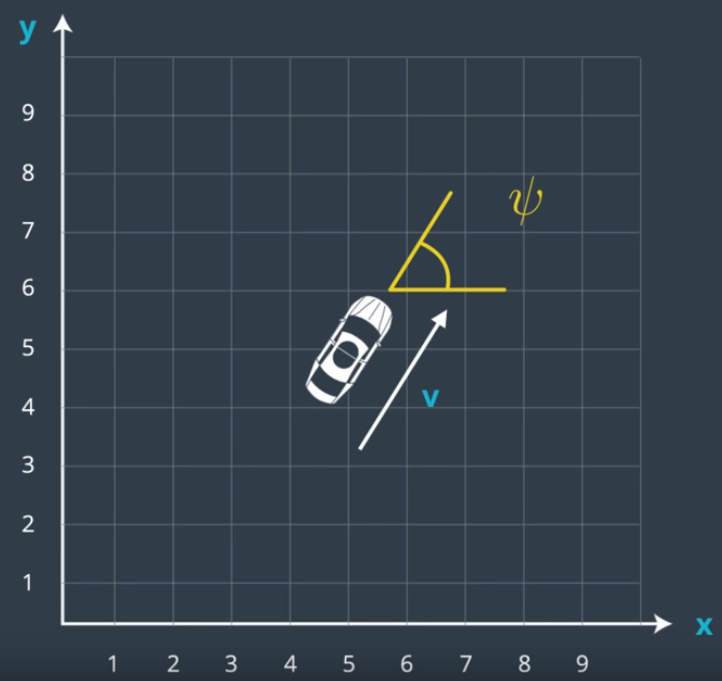
\includegraphics[width=0.5\textwidth]{state}
    \caption{Model state}
    \label{fig:state}
\end{figure}
\FloatBarrier

\begin{itemize}
\item $x$: x position
\item $y$: y position
\item $\psi$: angle between speed vector and x-axis
\item $v$: speed vector
\end{itemize}

\subsubsection{Deriving the kinematic model}


Our state vector is $$ S_t = [x_t, y_t, \psi_t, v_t] $$

We derive an approximation model, kinematic, relating $S_{t+1}$ and $S_t$. The smaller the $dt$ the more accurate the model. \\

\textbf{Linear movement approximation}: assuming during $dt$ that $v_t$ and $\psi_t$ are constant:
$$ x_{t+1} = x_t + v_t * \cos(\psi_t) *  dt $$
$$ y_{t+1} = y_t + v_t * \sin(\psi_t) *  dt $$

\textbf{Rotational movement approximation}: assuming during $dt$ that $v_t$ and steering angle $\delta_t$ are constant:

$$ {M_{t+1}M_{t}} = \rho * (\psi_{t+1} - \psi_t) = v_t * dt$$
$$ \tan(\delta_t) = L_f / \rho $$
So we have:
$$ \psi_{t+1} = \psi_t + (v_t /\rho) * dt$$
$$ \psi_{t+1} = \psi_t + (v_t / L_f) * \tan(\delta_t) * dt $$
\textit{Note that for small $\delta_t$ we have $\tan(\delta_t) \approx \delta_t$} \\

\textbf{Speed update}: assuming during $dt$ that $a_t$ is constant:
$$ v_{t+1} = v_t + a_t * dt $$ \\

So to summarize our kinematic model is:

$$ x_{t+1} = x_t + v_t * \cos(\psi_t) *  dt $$
$$ y_{t+1} = y_t + v_t * \sin(\psi_t) *  dt $$
$$ \psi_{t+1} = \psi_t + (v_t / L_f) * \tan(\delta_t) * dt $$
$$ v_{t+1} = v_t + a_t * dt $$

The state vector is $ S_t = [x_t, y_t, \psi_t, v_t] $. \\
The actuator command $ A_t = [ a_t, \delta_t ] $ defines a \textbf{constraint} between $S_{t+1}$ and $ S_t $.


\subsubsection{Errors}

The errors variables are the following:
\begin{figure}[h]
    \centering
    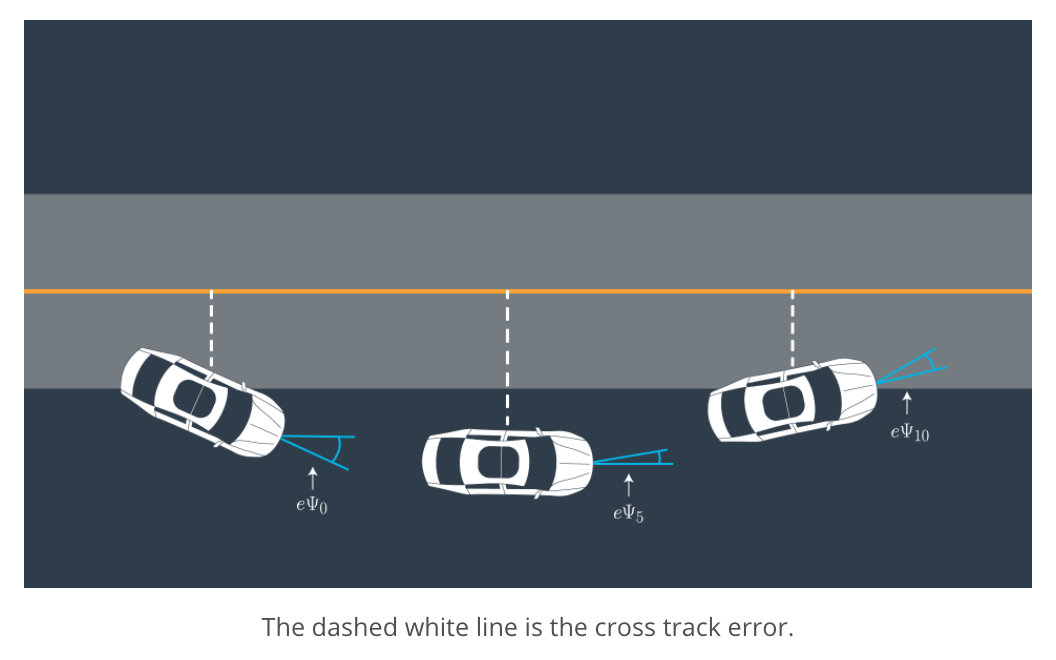
\includegraphics[width=0.75\textwidth]{errors}
    \caption{Model errors}
    \label{fig:errors}
\end{figure}
\FloatBarrier

\begin{itemize}
\item $cte$: cross track error. It corresponds to distance of vehicle from the planned trajectory (as planned by path planning module)
\item $e\Psi$: psie error is the angle difference of the vehicle trajectory with the planned trajectory (as planned by path planning module)
\end{itemize}

\textbf{The new state vector is $[x_t, y_t, \psi_t, v_t, cte_t, e\Psi_t]$.
}
\subsubsection{Kinematic Model}


\subsection{Dynamic Models}


Forces, Slip Angle, Slip ratio and Tire Models


\section{Model Predictive Control}

MPC reframes the task of following a trajectory as an optimization problem. The solution to the optimization problem is the optimal trajectory. \\

MPC involves simulating different actuator inputs, predicting the resulting trajectory and minimizing a set of constraints (or cost functions). \\ 

\textbf{Input:} a reference trajectory we want to follow \\ \\
\textbf{Constraints:}
\begin{itemize}
\item Vehicle Model
\item Comfort
\end{itemize}

\textbf{Output:} actuator commands (steering, throttling, braking ...)  \\ \\

Once we found the lowest cost trajectory, we implement the very first set of actuation commands. Then we throw away the rest of the trajectory we calculated. Instead of using the old trajectory we predicted, we take our new state and use that to calculate a new optimal trajectory. In that sense, we are constantly calculating inputs over a future horizon. That's why this approach is also called Receding Horizon Control. We constantly reevaluate the trajectory because our vehicle model is not perfect and the next predicted (or planned) state may (slightly...) differ with our prediction (in the sense of a consequence of a command sent). 


\begin{figure}[h]
    \centering
    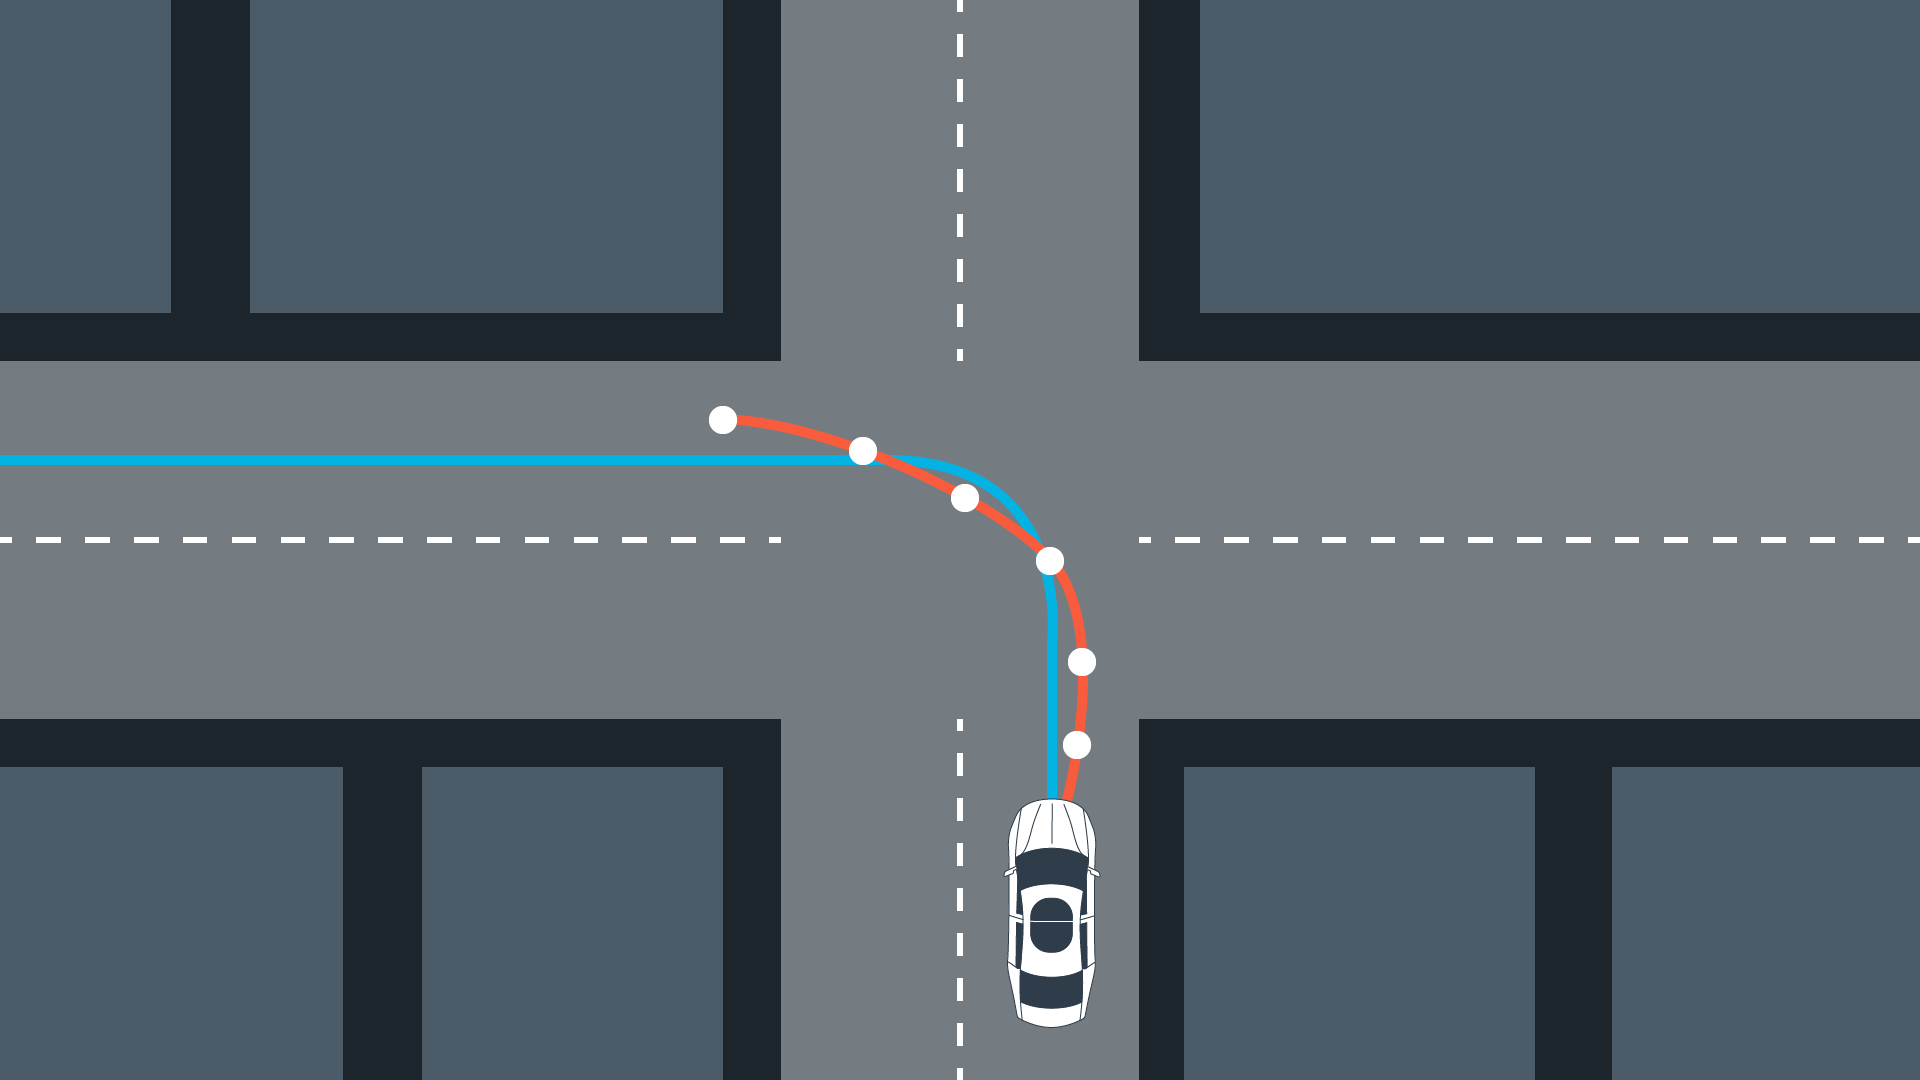
\includegraphics[width=0.5\textwidth]{minimization}
    \caption{Minimization problem}
    \label{fig:minimization}
\end{figure} 

\subsection{Optimization under constraints: cost functions}

\subsection{Timsestep length and Elapsed duration}

N=10 and dt=100 ms are used so that we are working on 1 second of data.
This is a trade-off: we need enough data visibility to ensure a good prediction, but we also have to limit the amount of computation.
In general, smaller dt gives better accuracy, but that will require higher N for given horizon (N*dt). However, increasing N will result in longer computational time which increases the latency. The most common choice of values is N=10 and dt=0.1 but anything between N=20, dt=0.05 should work.

\begin{figure}[h]
    \centering
    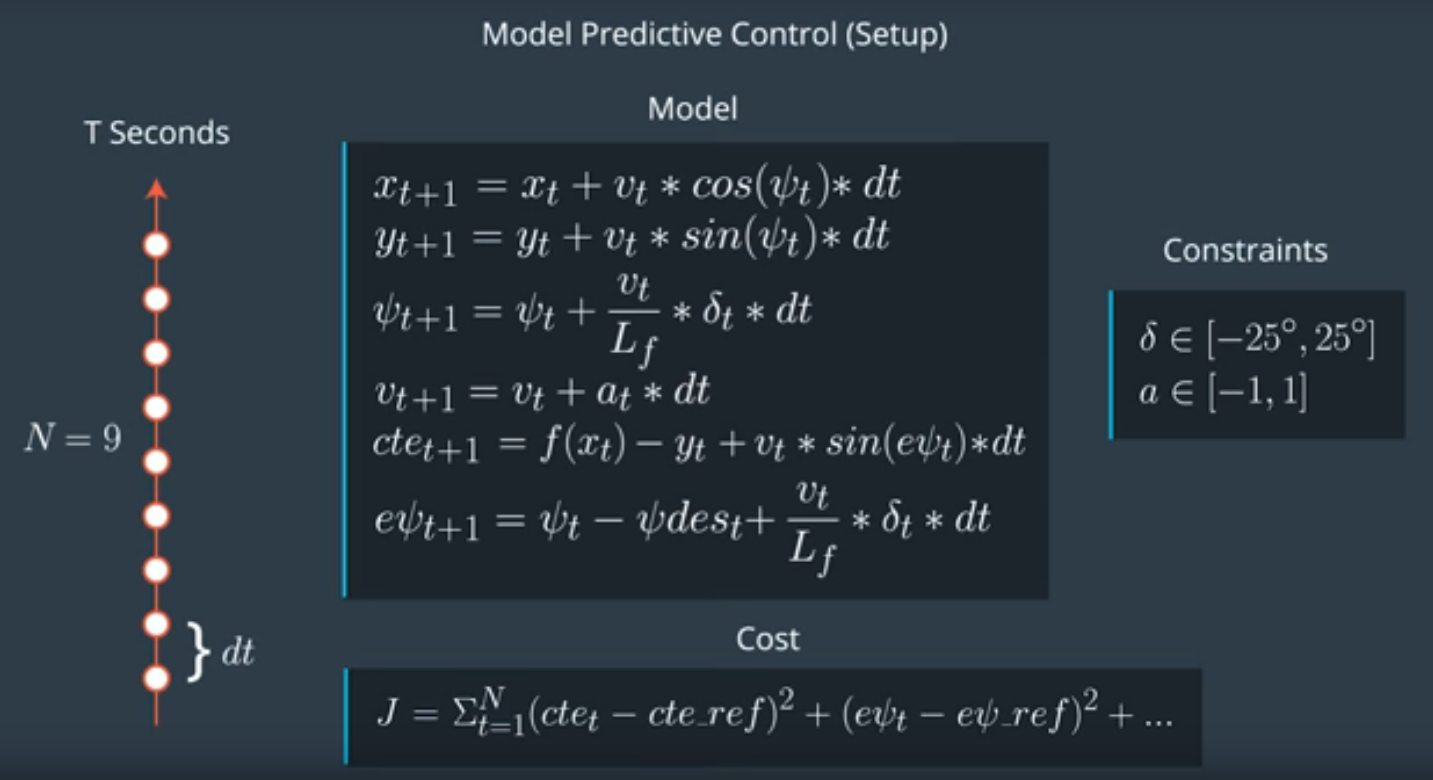
\includegraphics[width=0.75\textwidth]{solver_setup}
    \caption{Solver setup with N*dt time horizon}
    \label{fig:solver_setup}
\end{figure}

\subsection{Latency handling}


A contributing factor to latency is actuator dynamics. For example the time elapsed between when you command a steering angle to when that angle is actually achieved. This could easily be modeled by a simple dynamic system and incorporated into the vehicle model. One approach would be running a simulation using the vehicle model starting from the current state for the duration of the latency. The resulting state from the simulation is the new initial state for MPC.

Thus, MPC can deal with latency much more effectively, by explicitly taking it into account, than a PID controller.

\subsection{MPC Solver algorithm}

\begin{figure}[h]
    \centering
    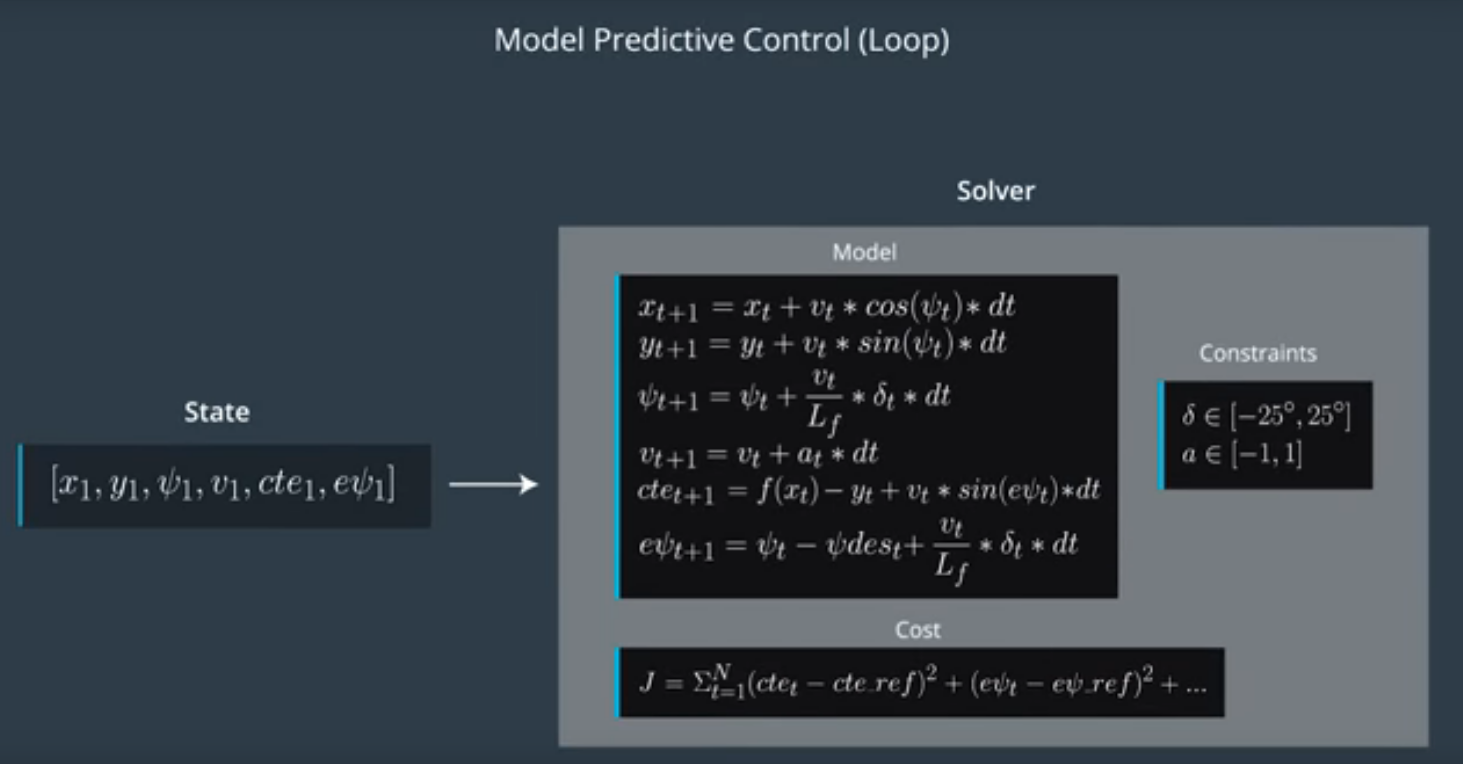
\includegraphics[width=0.75\textwidth]{solver_in}
    \caption{Solver input}
    \label{fig:solver_in}
\end{figure}

\begin{figure}[h]
    \centering
    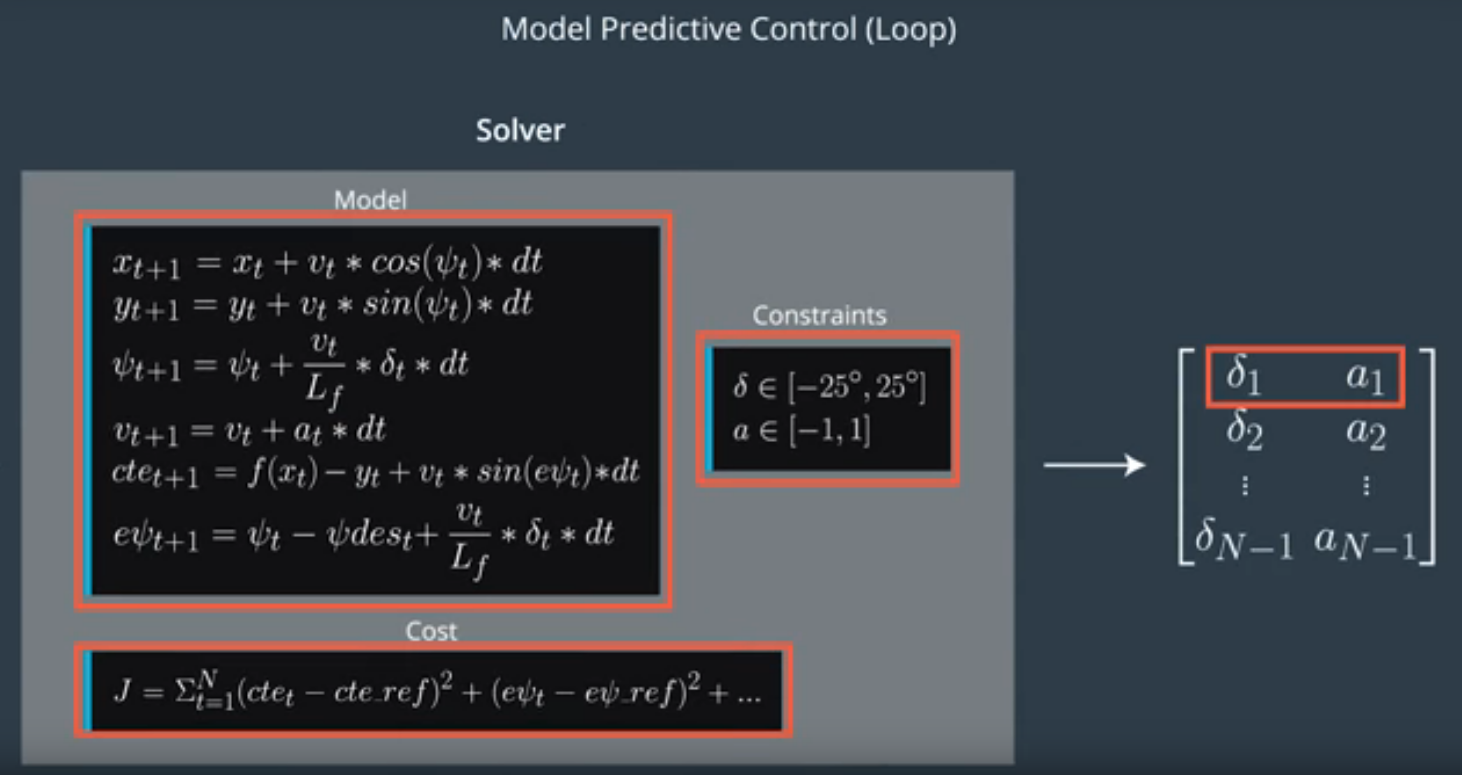
\includegraphics[width=0.75\textwidth]{solver_out}
    \caption{Solver output}
    \label{fig:solver_out}
\end{figure}

\begin{figure}[h]
    \centering
    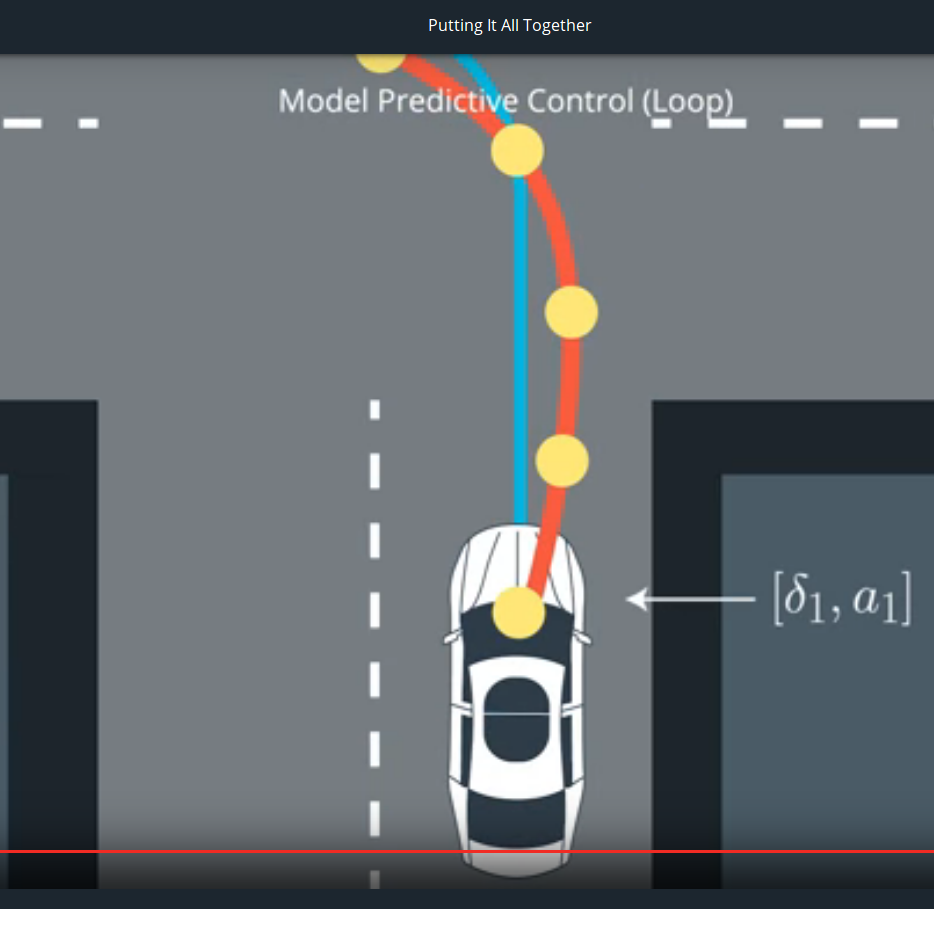
\includegraphics[width=0.5\textwidth]{solver_actuate}
    \caption{Solver actuator commands}
    \label{fig:solver_actuate}
\end{figure}

\FloatBarrier

\subsection{MPC Solver code}

\begin{lstlisting}[language=C++, caption={MPC solver with ipopt}]
#include "MPC.h"
#include <cppad/cppad.hpp>
#include <cppad/ipopt/solve.hpp>
#include "Eigen-3.3/Eigen/Core"
#include "Eigen-3.3/Eigen/QR"

using CppAD::AD;

// TODO: Set the timestep length and duration
size_t N = 10;
double dt = 0.1;

// This value assumes the model presented in the classroom is used.
//
// It was obtained by measuring the radius formed by running the vehicle in the
// simulator around in a circle with a constant steering angle and velocity on a
// flat terrain.
//
// Lf was tuned until the the radius formed by the simulating the model
// presented in the classroom matched the previous radius.
//
// This is the length from front to CoG that has a similar radius.
const double Lf = 2.67;

// NOTE: feel free to play around with this
// or do something completely different

double ref_v = 120;

// The solver takes all the state variables and actuator
// variables in a singular vector. Thus, we should to establish
// when one variable starts and another ends to make our lifes easier.
size_t x_start = 0;
size_t y_start = x_start + N;
size_t psi_start = y_start + N;
size_t v_start = psi_start + N;
size_t cte_start = v_start + N;
size_t epsi_start = cte_start + N;
size_t delta_start = epsi_start + N;
size_t a_start = delta_start + N - 1;

class FG_eval {
 public:
  // Fitted polynomial coefficients
  Eigen::VectorXd coeffs;
  FG_eval(Eigen::VectorXd coeffs) { this->coeffs = coeffs; }

  typedef CPPAD_TESTVECTOR(AD<double>) ADvector;
  void operator()(ADvector& fg, const ADvector& vars) {
    // TODO: implement MPC
    // `fg` a vector of the cost constraints, `vars` is a vector of variable values (state & actuators)
    // NOTE: You'll probably go back and forth between this function and
    // the Solver function below.

    // The cost is stored is the first element of `fg`.
    // Any additions to the cost should be added to `fg[0]`.
    fg[0] = 0;

    // Reference State Cost
    // TODO: Define the cost related the reference state and
    // any anything you think may be beneficial.
    for (size_t t = 0; t < N; t++) {
      fg[0] += 4 * 2000 * CppAD::pow(vars[cte_start + t], 2);
      fg[0] += 4 * 2000 * CppAD::pow(vars[epsi_start + t], 2);
      fg[0] += CppAD::pow(vars[v_start + t] - ref_v, 2);
    }

    // Minimize the use of actuators.
    for (size_t t = 0; t < N - 1; t++) {
      fg[0] += 5 * CppAD::pow(vars[delta_start + t], 2);
      fg[0] += 5 * CppAD::pow(vars[a_start + t], 2);
    }

    // smooth
    for (size_t t = 0; t < N - 2; t++) {
      fg[0] += 200 * CppAD::pow(vars[delta_start + t + 1] - vars[delta_start + t], 2);
      fg[0] += 10 * CppAD::pow(vars[a_start + t + 1] - vars[a_start + t], 2);
    }

    //
    // Setup Constraints
    //
    // NOTE: In this section you'll setup the model constraints.

    // Initial constraints
    //
    // We add 1 to each of the starting indices due to cost being located at
    // index 0 of `fg`.
    // This bumps up the position of all the other values.
    fg[1 + x_start] = vars[x_start];
    fg[1 + y_start] = vars[y_start];
    fg[1 + psi_start] = vars[psi_start];
    fg[1 + v_start] = vars[v_start];
    fg[1 + cte_start] = vars[cte_start];
    fg[1 + epsi_start] = vars[epsi_start];

    // The rest of the constraints
    for (size_t t = 1; t < N; t++) {
      // at time t+1
      AD<double> x1 = vars[x_start + t];
      AD<double> y1 = vars[y_start + t];
      AD<double> psi1 = vars[psi_start + t];
      AD<double> v1 = vars[v_start + t];
      AD<double> cte1 = vars[cte_start + t];
      AD<double> epsi1 = vars[epsi_start + t];

      // at time t
      AD<double> x0 = vars[x_start + t - 1];
      AD<double> y0 = vars[y_start + t - 1];
      AD<double> psi0 = vars[psi_start + t - 1];
      AD<double> v0 = vars[v_start + t - 1];
      AD<double> cte0 = vars[cte_start + t - 1];
      AD<double> epsi0 = vars[epsi_start + t - 1];

      AD<double> delta0 = vars[delta_start + t - 1];
      AD<double> a0 = vars[a_start + t - 1];

      // XXX: to be updated
      AD<double> f0 = coeffs[0] + coeffs[1] * x0 + coeffs[2] * x0 * x0 + coeffs[3] * x0 * x0 * x0;
      AD<double> psides0 = CppAD::atan(coeffs[1] + 2 * coeffs[2] * x0 + 3 * coeffs[3] * x0 * x0);

      // Here's `x` to get you started.
      // The idea here is to constraint this value to be 0.
      //
      // NOTE: The use of `AD<double>` and use of `CppAD`!
      // This is also CppAD can compute derivatives and pass
      // these to the solver.

      // TODO: Setup the rest of the model constraints
      fg[1 + x_start + t] = x1 - (x0 + v0 * CppAD::cos(psi0) * dt);
      fg[1 + y_start + t] = y1 - (y0 + v0 * CppAD::sin(psi0) * dt);
      fg[1 + psi_start + t] = psi1 - (psi0 - v0 * delta0 / Lf * dt); // XXX + -> - (as received from simulator)
      fg[1 + v_start + t] = v1 - (v0 + a0 * dt);

      // BUG fg[1 + cte_start + t] = cte1 - (cte0 + v0 * CppAD::sin(epsi0) * dt);
      // BUG fg[1 + epsi_start + t] = epsi1 - (epsi0 + v0 * delta0 / Lf * dt);
      fg[1 + cte_start + t] = cte1 - ((f0 - y0) + (v0 * CppAD::sin(epsi0) * dt));
      fg[1 + epsi_start + t] = epsi1 - ((psi0 - psides0) - v0 * delta0 / Lf * dt); // XXX + -> -
    }
  }
};

//
// MPC class definition implementation.
//
MPC::MPC() {}
MPC::~MPC() {}

vector<double> MPC::Solve(Eigen::VectorXd state, Eigen::VectorXd coeffs) {
  bool ok = true;
  size_t i;
  typedef CPPAD_TESTVECTOR(double) Dvector;

  double x = state[0];
  double y = state[1];
  double psi = state[2];
  double v = state[3];
  double cte = state[4];
  double epsi = state[5];

  // TODO: Set the number of model variables (includes both states and inputs).
  // For example: If the state is a 4 element vector, the actuators is a 2
  // element vector and there are 10 timesteps. The number of variables is:
  //
  // 4 * 10 + 2 * 9
  size_t n_vars = N * 6 + (N - 1) * 2;
  // TODO: Set the number of constraints
  size_t n_constraints = N * 6;

  // Initial value of the independent variables.
  // Should be 0 except for the initial values.
  Dvector vars(n_vars);
  for (i = 0; i < n_vars; i++) {
    vars[i] = 0.0;
  }
  // Set the initial variable values
  vars[x_start] = x;
  vars[y_start] = y;
  vars[psi_start] = psi;
  vars[v_start] = v;
  vars[cte_start] = cte;
  vars[epsi_start] = epsi;

  // Lower and upper limits for x
  Dvector vars_lowerbound(n_vars);
  Dvector vars_upperbound(n_vars);
  // TODO: Set lower and upper limits for variables.
  // Set all non-actuators upper and lowerlimits
  // to the max negative and positive values.
  for (i = 0; i < delta_start; i++) {
    vars_lowerbound[i] = -1.0e19;
    vars_upperbound[i] = 1.0e19;
  }

  // The upper and lower limits of delta are set to -25 and 25
  // degrees (values in radians).
  // NOTE: Feel free to change this to something else.
  for (i = delta_start; i < a_start; i++) {
    vars_lowerbound[i] = -0.436332 * Lf; // *Lf ? XXX
    vars_upperbound[i] = 0.436332 * Lf;  // *Lf ?
  }

  // Acceleration/decceleration upper and lower limits.
  // NOTE: Feel free to change this to something else.
  for (i = a_start; i < n_vars; i++) {
    vars_lowerbound[i] = -1.0;
    vars_upperbound[i] = 1.0;
  }


  // Lower and upper limits for the constraints
  // Should be 0 besides initial state.
  Dvector constraints_lowerbound(n_constraints);
  Dvector constraints_upperbound(n_constraints);
  for (i = 0; i < n_constraints; i++) {
    constraints_lowerbound[i] = 0;
    constraints_upperbound[i] = 0;
  }
  constraints_lowerbound[x_start] = x;
  constraints_lowerbound[y_start] = y;
  constraints_lowerbound[psi_start] = psi;
  constraints_lowerbound[v_start] = v;
  constraints_lowerbound[cte_start] = cte;
  constraints_lowerbound[epsi_start] = epsi;

  constraints_upperbound[x_start] = x;
  constraints_upperbound[y_start] = y;
  constraints_upperbound[psi_start] = psi;
  constraints_upperbound[v_start] = v;
  constraints_upperbound[cte_start] = cte;
  constraints_upperbound[epsi_start] = epsi;

  // Object that computes objective and constraints
  FG_eval fg_eval(coeffs);

  //
  // NOTE: You don't have to worry about these options
  //
  // options for IPOPT solver
  std::string options;
  // Uncomment this if you'd like more print information
  options += "Integer print_level  0\n";
  // NOTE: Setting sparse to true allows the solver to take advantage
  // of sparse routines, this makes the computation MUCH FASTER. If you
  // can uncomment 1 of these and see if it makes a difference or not but
  // if you uncomment both the computation time should go up in orders of
  // magnitude.
  options += "Sparse  true        forward\n";
  options += "Sparse  true        reverse\n";
  // NOTE: Currently the solver has a maximum time limit of 0.5 seconds.
  // Change this as you see fit.
  options += "Numeric max_cpu_time          0.5\n";

  // place to return solution
  CppAD::ipopt::solve_result<Dvector> solution;

  // solve the problem
  CppAD::ipopt::solve<Dvector, FG_eval>(
      options, vars, vars_lowerbound, vars_upperbound, constraints_lowerbound,
      constraints_upperbound, fg_eval, solution);

  //
  // Check some of the solution values
  ok &= solution.status == CppAD::ipopt::solve_result<Dvector>::success;

  // Cost
  auto cost = solution.obj_value;
  //std::cout << "Cost " << cost << std::endl;

  // TODO: Return the first actuator values. The variables can be accessed with
  // `solution.x[i]`.
  //
  // {...} is shorthand for creating a vector, so auto x1 = {1.0,2.0}
  // creates a 2 element double vector.
  //return {solution.x[delta_start],   solution.x[a_start]};

  vector<double> result;

  result.push_back(solution.x[delta_start]);
  result.push_back(solution.x[a_start]);

  for (size_t i = 0; i < N - 1; i++) {
    result.push_back(solution.x[x_start + i + 1]);
    result.push_back(solution.x[y_start + i + 1]);
  }

  return result;
}
\end{lstlisting}

\end{document}}